% Retained method diagnostics from the previous manuscript: E1, E5, E6.
\label{sec:ablation-studies}

We report three diagnostic studies on ResNet-50/CIFAR-10.
Test accuracies are measured on the official test set after
validation-based checkpoint selection. The comparisons are exploratory:
their outcomes informed subsequent experiments. Each comparison has
its own architecture and training protocol, as specified below.
Figure~\ref{fig:resnet-cifar-ablations} summarizes these studies.

\begin{figure*}[t]
  \centering
  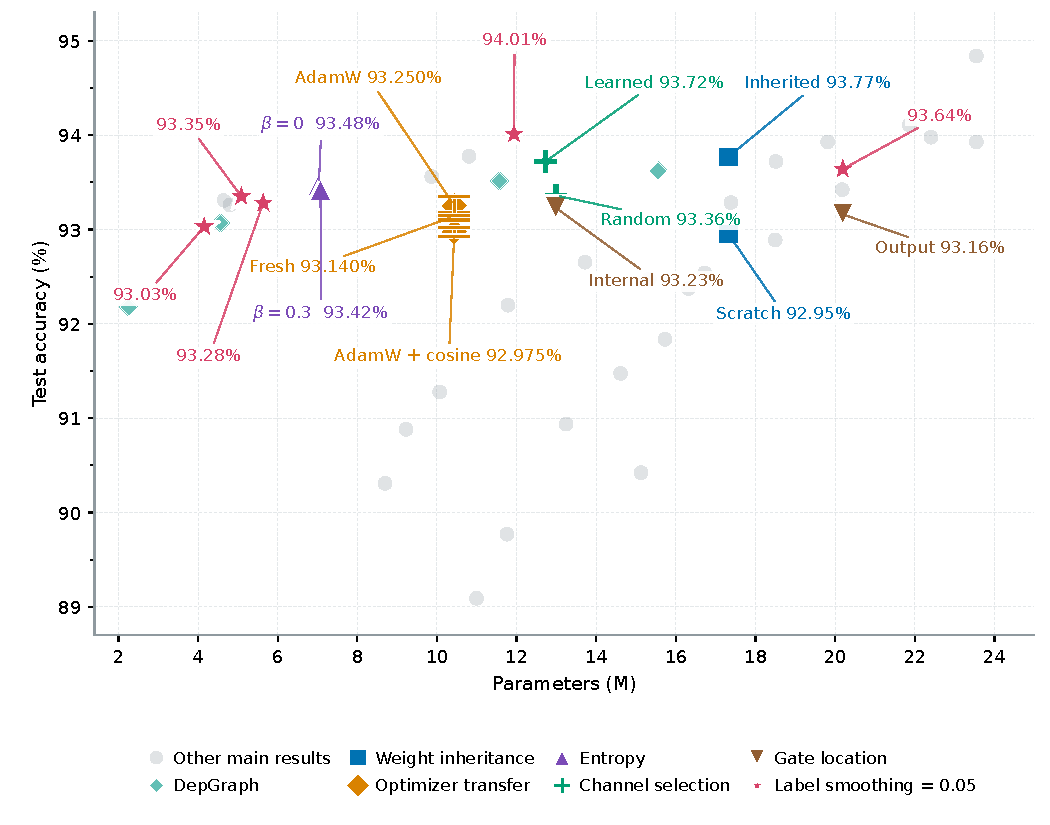
\includegraphics[width=\textwidth]{figures/resnet50_cifar10_ablations.pdf}
  \caption{Three ResNet-50/CIFAR-10 diagnostics. Labels give physical
    parameter counts. Only the weight-initialization pair fixes the
    architecture and search checkpoint; selection and gate-placement
    comparisons use different architectures or training protocols.}
  \label{fig:resnet-cifar-ablations}
  \Description{Three panels compare inherited and random weights,
    adaptive and historical random selection recipes, and internal and
    output gates. No uncertainty intervals are implied.}
\end{figure*}


% E1
\paragraph{Weight inheritance.}
We fix a pruned architecture with 17{,}321{,}706 parameters and
compare inherited and randomly initialized weights. Both branches
use the same 60-epoch search result followed by 90 epochs of recovery.
Inherited weights reach 93.77\% test accuracy, compared with
92.95\% from random initialization, a difference of
0.82 percentage points (Table~\ref{tab:ablation-weights}).
This result concerns one selected architecture and one search result;
it does not establish an advantage across architectures or training seeds.

\begin{table}[t]
  \centering
  \caption{Recovery initialization for a fixed architecture.
    Accuracy is reported in percent.}
  \label{tab:ablation-weights}
  \begin{tabular}{@{}lrr@{}}
    \toprule
    Initialization & Validation & Test \\
    \midrule
    Inherited weights & 94.38 & 93.77 \\
    Random weights & 93.82 & 92.95 \\
    \bottomrule
  \end{tabular}
\end{table}
% E2
% \paragraph{Optimizer and scheduler state transfer.}
% For a separate, fixed 10{,}435{,}943-parameter architecture, we compare
% three recovery policies from a common search checkpoint, with a
% 60/90 search/recovery split and two recovery repetitions per policy.
% With a restarted cosine schedule, transferring AdamW states gives
% 93.250\% mean test accuracy, compared with 93.140\% using fresh
% states (Table~\ref{tab:ablation-optimizer}). This 0.11-point difference
% changes sign between repetitions. Continuing the cosine schedule
% with transferred AdamW states gives 92.975\%, 0.275 points below
% restarting it. Two recovery repetitions do not support a strong
% statistical conclusion.

% \begin{table}[t]
%   \centering
%   \caption{Test accuracy (\%) for state-transfer policies.
%     The mean is computed over the two recovery repetitions.}
%   \label{tab:ablation-optimizer}
%   \small
%   \setlength{\tabcolsep}{3pt}
%   \begin{tabular}{@{}llrrr@{}}
%     \toprule
%     AdamW & Cosine & Rep.~1 & Rep.~2 & Mean \\
%     \midrule
%     Fresh & Restarted & 93.18 & 93.10 & 93.140 \\
%     Transferred & Restarted & 93.15 & 93.35 & 93.250 \\
%     Transferred & Continued & 92.93 & 93.02 & 92.975 \\
%     \bottomrule
%   \end{tabular}
% \end{table}
% % E4
% \paragraph{Entropy regularization at similar sizes.}
% We compare two runs with $\beta=0$ and $\beta=0.3$, retrospectively
% selected for their similar physical parameter counts. Both use
% 60 epochs of search, 90 epochs of recovery, adaptive $\lambda$,
% and the same accuracy tolerances and selector based on the expected
% open count.
% The $\beta=0$ model reaches 93.48\% test accuracy at 7.034M
% parameters; the $\beta=0.3$ model reaches 93.42\% at 7.073M
% (Table~\ref{tab:ablation-entropy}). The observed difference is
% 0.06 percentage points. These single-seed runs come from different
% series and code revisions and have different architectures and MAC
% counts, so the pair does not isolate the effect of entropy regularization.

% \begin{table}[t]
%   \centering
%   \caption{Entropy comparison using physical deployment sizes.
%     Accuracy is in percent; M and G denote millions and billions.}
%   \label{tab:ablation-entropy}
%   \small
%   \setlength{\tabcolsep}{4pt}
%   \begin{tabular}{@{}rrrrr@{}}
%     \toprule
%     $\beta$ & Params (M) & MACs (G) & Validation & Test \\
%     \midrule
%     0 & 7.034 & 0.538 & 93.92 & 93.48 \\
%     0.3 & 7.073 & 0.503 & 93.96 & 93.42 \\
%     \bottomrule
%   \end{tabular}
% \end{table}
% E5
\paragraph{Comparison with random channel selection.}
A separate later adaptive run reaches 93.72\% test accuracy with
12.728M parameters, compared with 93.36\% at 12.984M for a
historical random-selection control (Table~\ref{tab:ablation-random}).
Both models use 150 training epochs, but the adaptive run uses a
single 60-epoch search followed by 90 epochs of recovery, whereas
the random control uses an earlier iterative protocol with fixed
$\lambda$. The random model also has fewer MACs: 0.692G versus
1.108G. The 0.36-point accuracy difference therefore compares
complete training recipes and does not isolate channel ranking
or adaptive sparsity scheduling.

\begin{table}[t]
  \centering
  \caption{Historical random control and the later adaptive recipe.
    Sizes describe physical models; test accuracy is in percent.}
  \label{tab:ablation-random}
  \small
  \setlength{\tabcolsep}{4pt}
  \begin{tabular}{@{}lrrr@{}}
    \toprule
    Method & Params (M) & MACs (G) & Test \\
    \midrule
    Random selection & 12.984 & 0.692 & 93.36 \\
    Our adaptive recipe & 12.728 & 1.108 & 93.72 \\
    \bottomrule
  \end{tabular}
\end{table}
% E6
\paragraph{Internal and output channel gates.}
An earlier experiment uses fixed $\lambda=0.001$ and 150 training
epochs per model to compare gates on residual-branch outputs with
gates on internal bottleneck channels. Internal gating produces
12.983M parameters at 93.23\% test accuracy, compared with
20.189M at 93.16\% for output gating
(Table~\ref{tab:ablation-gate-location}). These runs demonstrate
a smaller model at similar accuracy, but their pruning budgets
and resulting architectures differ. They do not isolate gate
placement at a fixed size or evaluate adaptive scheduling.

\begin{table}[t]
  \centering
  \caption{Gate placement in the early fixed-$\lambda$ experiment.
    Accuracy is in percent and parameter counts are physical.}
  \label{tab:ablation-gate-location}
  \begin{tabular}{@{}lrrr@{}}
    \toprule
    Gate location & Params (M) & Validation & Test \\
    \midrule
    Branch output & 20.189 & 93.88 & 93.16 \\
    Bottleneck internal & 12.983 & 94.04 & 93.23 \\
    \bottomrule
  \end{tabular}
\end{table}

% E8: historical label-smoothed recovery; red stars in the working notebook.
% \paragraph{Label smoothing during recovery.}
% We additionally report five historical runs with label smoothing
% $\varepsilon_{\mathrm{LS}}=0.05$ during recovery
% (Table~\ref{tab:ablation-label-smoothing}). Search uses ordinary
% cross-entropy without label smoothing. Each run uses 60 epochs
% of adaptive mask search followed by 90 epochs of recovery,
% with seed~42, a minimum channel-retention ratio of 0.08 and
% entropy regularization disabled. The five runs use different
% accuracy tolerances and produce different pruned architectures.
% Among these five runs, the highest test accuracy is
% \textbf{94.01\%} with \textbf{11.934M} parameters; a smaller model reaches 93.35\%
% with 5.086M parameters.

% The search learning-rate floor is $6.6443\cdot10^{-4}$,
% compared with zero in the main series; there is also no
% separate BatchNorm recalibration before recovery.
% The results therefore characterize the complete training recipe;
% they do not isolate the effect of label smoothing alone.

% \begin{table}[t]
%   \centering
%   \caption{Historical runs with label smoothing 0.05 during
%     recovery. Parameter counts are physical; accuracy is measured
%     on the official CIFAR-10 test set.}
%   \label{tab:ablation-label-smoothing}
%   \begin{tabular}{@{}rr@{}}
%     \toprule
%     Parameters (M) & Test accuracy (\%) \\
%     \midrule
%     4.154 & 93.03 \\
%     5.086 & 93.35 \\
%     5.637 & 93.28 \\
%     \textbf{11.934} & \textbf{94.01} \\
%     20.192 & 93.64 \\
%     \bottomrule
%   \end{tabular}
% \end{table}
% % Points: notebooks/data/selected_parameter_curve_red_stars.csv, Ours (selected).
% % Test sources: user frozen-test report 2026-09-23 for the first three;
% % parameter_curve_target13m_17m_results.tar.gz/test_comparison.csv for the last two.
% % Actual phase configs: parameter_curve_4x150_results.tar.gz and the 13m/17m archive.
% % For approx9m_retry, recovery LS=.05 is reconstructed from its launch command
% % and parameter_curve_recovery90_ls005; the effective retry config was not retained.
% % Source audit: tasks/adhoc/pruning-accuracy-parameters-plot/
% % selected-red-star-runs.md and ours-selected-configuration-comparison.md.
